\chapter{Diagonalisation}
\label{chapter:Fr_27-diag}
 
Dans le chapitre précédent, nous avons défini les valeurs propres et les vecteurs propres d'une matrice carrée $A$ de taille $n\times n$.  À chaque valeur propre, nous associons sa \emph{multiplicité algébrique}, qui est sa multiplicité en tant que racine du polynôme caractéristique $\det(A-\lambda I_n)$ de $A$.  Nous associons également à chaque valeur propre sa \emph{multiplicité géométrique}, qui est la dimension de l'espace propre associé $E_\lambda$.  Le résultat clé (Théorème~\ref{thm:limitsmult}) est que pour chaque valeur propre $\lambda$ de $A$, on a
$$
1\, \leq\, \text{multiplicité géométrique de $\lambda$}\, \leq\,
\text{multiplicité algébrique de $\lambda$}.
$$
En particulier, la dimension de l'espace propre $E_\lambda$ ne peut \emph{jamais} être plus grande que la multiplicité algébrique de $\lambda$.



\section{À propos de la diagonalisation}\label{section:diag}

Rappelons la Définition \ref{diagble} :
On dit que la matrice $A$ de taille $n\times n$ est \defn{diagonalisable sur $\R$} s'il existe 
une base de $\R^n$ constituée exclusivement de vecteurs propres de $A$.
 

Nous avons vu la dernière fois que si $A$ admet $n$ valeurs propres réelles distinctes,
alors $A$ est nécessairement diagonalisable. De plus, dans certains cas favorables, il est aussi possible que  $A$ soit diagonalisable même
 en ayant des valeurs propres multiples (mais ce n'est pas toujours le cas).


\begin{myprob} Soit la matrice
$$
A = \mat{3 & 2 & 4\\ 2& 0 & 2\\ 4 & 2 & 3}\,.
$$
Trouvez les valeurs propres $A$ et déterminez une base pour chaque espace propre. En déduire 
si $A$ est diagonalisable ou non.

\begin{mysol}  Nous devons d'abord calculer les valeurs propres de $A$.  Commençons par calculer le polynôme caractéristique :
$$
\det( A-\lambda I_3) = 
\det \mat{
3-\lambda & 2      & 4 \\ 
2          & -\lambda & 2 \\ 
4          & 2      &  3-\lambda }\,.
$$
Bien qu'on puisse calculer directement le déterminant avec la définition, c'est plus facile et plus rapide de commencer par réduire par rapport aux lignes / colonnes pour faire apparaître des coefficients $0$. Faisons donc l'opération $-2 L_2 + L_3 \to L_3$, ce qui ne change pas
la valeur du déterminant :
$$
= \det \mat{
3-\lambda & 2      & 4 \\ 
2          & -\lambda & 2 \\ 
0          & 2+2 \lambda \,     &  - 1 -\lambda}
$$
et ensuite nous remarquons que l'entrée $(3,2)$ est le multiple par $-2$ de l'entrée 
$(3,3)$.  Donc, sachant que le déterminant d'une matrice
est le même que celui de sa transpos\'ee, nous pouvons effectuer l'opération suivante sur la $2$e colonne :
$2C_3+C_2\to C_2$; et cela ne changera pas non plus la valeur du déterminant :
$$
=  \det \mat{
3-\lambda & 10      & 4 \\ 
2          & 4-\lambda & 2 \\ 
0          & 0 \,     &  - 1 -\lambda}\,.
$$
Enfin, faisons le développement de Laplace selon la 3e ligne pour avoir
une réponse partiellement déjà factorisée:
$$
=-(\lambda + 1) \left( (3-\lambda)(  4-\lambda) - 20 \right) = -(\lambda + 1)(\lambda^2 - 7 \lambda -8) = -(\lambda+1)^2(\lambda - 8)\,.
$$
C'est le polynôme caractéristique de $A$.


On en déduit que la matrice $A$ admet exactement deux valeurs propres : $-1$ avec multiplicité algébrique $2$,  et $8$ avec
multiplicité algébrique $1$.

Nous devons ensuite trouver une base pour chaque espace propre $E_{-1}$ et $E_8$.

Commençons avec $\lambda = 8$. On veut trouver l'expression de $E_8 = \ker(A-8I_3)$, donc on r\'eduit la matrice suivante :
$$
A-8I_n=\mat{-5 &  2      & 4 \\ 
2          & -8 & 2 \\ 
4          & 2      & -5}
\sim  
\mat{
1 & -4 & 1\\
5 & -2 & -4\\
-4 & -2 & 5}
\sim
\mat{
1 & -4 & 1\\
0 & 18 & -9\\
0 & -18 & 9}
$$
$$
\sim \mat{1 & -4 & 1\\
0 & 1 & -\frac12 \\
0 & 0 & 0}
\sim
\mat{1 & 0 & -1\\ 0 & 1 & -\frac12 \\ 0 & 0 & 0}\,.
$$
On voit qu'il n'y a qu'une seule variable libre (la troisième), donc $\dim(E_8)=\dim \ker(A-8I_n) =1$. La multiplicité géométrique de $8$ est donc $1$. (On pouvait s'y attendre par l'inégalité qu'on a citée en début de chapitre !)
Une base pour $E_8$ est $\{(1,\frac12, 1)\}$, ou $\{(2,1,2)\}$ si vous
préférez enlever les fractions.


Ensuite, attaquons-nous à $\lambda =-1$. Pour trouver l'expression de $E_{-1} = \ker(A-(-I_3))=\ker(A+I_3)$, nous réduisons la matrice suivante :
$$
A+I_3=\mat{4 & 2              & 4 \\ 
2          & 1         & 2 \\ 
4          & 2     & 4}
\sim
\mat{1 & \frac12 & 1\\ 0 & 0 & 0\\ 0 & 0 & 0}\,.
$$
On voit que l'on a deux variables libres (les deux dernières colonnes), donc la multiplicité géométrique de $-1$ est $2$: $\dim(E_{-1}) = 2$. Ceci coïncide avec
la multiplicité algébrique de $-1$, donc c'est une bonne chose : on va pouvoir trouver une base de vecteurs propres de $\R^3$.  En tout cas, une base de $E_{-1}$ est donnée par exemple par :
$$
\{ (-{\textstyle\frac12}, 1, 0) , (-1, 0, 1)\}
$$
(ou multipliez le premier par 2 si vous préférez, pour obtenir $\{ (-1, 2, 0), (-1,0,1)\}$).


Finalement, on remarque que l'ensemble
$$
\{ (2,1,2), (-1,2,0), (-1,0,1)\}
$$
est linéairement indépendant (c'est le cas par le Théorème \ref{theo: Les vecteurs propres sont LI quand les valeurs propres sont distinctes}, mais vérifiez-le !) et donc forme une base pour 
$\R^3$ puisqu'il contient exactement trois éléments LI. En conclusion, comme $\R^3$ admet bien une base entièrement constituée de vecteurs propres
de $A$, on en déduit que $A$ est bien diagonalisable. D'où le résultat.
\end{mysol}\end{myprob}

\medskip
Et alors? Quel est l'intérêt au final d'avoir une matrice diagonalisable ?

Continuons avec l'exemple précédent. Étant donnée une matrice $A =  \scriptsize\mat{3 & 2 & 4\\ 2& 0 & 2\\ 4 & 2 & 3}$ comme ci-dessus, construisons
la matrice $P$ dont les colonnes sont les vecteurs propres qu'on a choisi pour constituer des bases des espaces propres de $A$ :
$$
P = \mat{2 & -1 & -1 \\ 1 & 2 & 0\\ 2 & 0 & 1}\,.
$$
Puisque ses colonnes forment une base pour $\R^3$, on sait que $P$ est inversible (cf. le Grand Théorème, avec les multiples propriétés équivalentes).  Appelons ces
colonnes respectivement $\vv_1, \vv_2, \vv_3$.
Alors :
\begin{align*}
AP &= A\mat{\vv_1 & \vv_2 & \vv_3} \\
&=  \mat{A\vv_1 & A\vv_2 & A\vv_3}\\
&= \mat{8\vv_1 & (-1)\vv_2 & (-1)\vv_3}\\
&= \mat{\vv_1 & \vv_2 & \vv_3}\mat{8 & 0 & 0\\ 0 & -1 & 0\\ 0 & 0 & -1}\\
&= PD\,,
\end{align*}
où $D = \scriptsize \mat{8 & 0 & 0\\ 0 & -1 & 0\\ 0 & 0 & -1}$ est la matrice diagonale constituée des valeurs propres de $A$
(données dans le {\it même ordre} que les vecteurs propres de $P$).

Puisque $P$ est inversible, alors on peut r\'e\'ecrire ceci comme:
$$
 P^{-1}AP=D\qquad \text{ ou encore }\qquad A = PDP^{-1}\,.
$$

\begin{proposition}[Diagonaliser une matrice]\index{diagonaliser une matrice}
Si $P$ est une matrice dont les colonnes sont des vecteurs propres 
de $A$ et forment une base de $\R^n$, et $D$ est la matrice diagonale dont les éléments diagonaux
sont les valeurs propres correspondantes aux vecteurs propres dans $P$ (dans le même ordre), alors
$$
 P^{-1}AP=D\qquad \text{ ou encore }\qquad A = PDP^{-1}.
$$
\end{proposition}

\begin{myprob}
Étant donnée la même matrice $A$ que dans l'exercice pr\'ec\'edent, calculez $A^n$, pour $n$ un entier naturel quelconque. 

\begin{mysol}
Pour avoir une id\'ee, essayons avec $n=5$ d'abord.
Comme $A = PDP^{-1}$, on a 
$$
A^5 = AAAAA = (PDP^{-1})(PDP^{-1})(PDP^{-1})(PDP^{-1})(PDP^{-1}) = PD^5P^{-1}\,.
$$
Ensuite, puisque $D$ est une matrice diagonale, le calcul de ses puissances est facile :
$$
D^5 = \mat{8 & 0 & 0\\  0 & -1 & 0\\ 0 & 0 & -1}^5 = 
\mat{8^5 & 0 & 0\\ 0 & (-1)^5 & 0 \\ 0 & 0 & (-1)^5}
= \mat{32\, 768 & 0 & 0\\  0 & -1 & 0\\ 0 & 0 & -1}\,.
$$
De même, de façon plus générale, on a $A^n = PD^n P^{-1}$ et $D^n$ est la matrice diagonale
dont les entrées diagonales sont $8^n$, puis $(-1)^n$, puis $(-1)^n$.\footnote{Ce résultat se montre par un raisonnement par récurrence.}

Un petit calcul donne $P^{-1}$ :
$$
P^{-1} = \frac19 \mat{2&1&2\\-1&4&-1\\-4&-2&5}\,,
$$
et donc 
$$
A^5 = \mat{2 & -1 & -1 \\ 1 & 2 & 0\\ 2 & 0 & 1}\mat{8^5 & 0 & 0\\ 0 & (-1)^5 & 0 \\ 0 & 0 & (-1)^5}\frac19 \mat{2&1&2\\-1&4&-1\\-4&-2&5}\,.
$$
De même pour $A^n$, pour tout $n$, mais en version légèrement plus désagréable :
$$
A^n = \mat{2 & -1 & -1 \\ 1 & 2 & 0\\ 2 & 0 & 1}\mat{8^n & 0 & 0\\ 0 & (-1)^n & 0 \\ 0 & 0 & (-1)^n}\frac19 \mat{2&1&2\\-1&4&-1\\-4&-2&5}\,.
$$
(Remarque : comme $A$ est inversible (v\'erifiez-le !), on peut m\^eme prendre $n$ négatif, et la même formule marchera aussi !\!!)
\end{mysol} \end{myprob}


L'équation $A = PDP^{-1}$ est la raison pour laquelle nous appelons ce processus \og diagonalisation\ \fg, parce qu'on peut passer de $A$ à une matrice diagonale $D$ en \emph{conjuguant} par la matrice $P$.
Des applications comme le calcul de l'expression de $A^n$ sont très importantes : elles figurent parmi les principales raisons qui motivent la diagonalisation.

Autre application importante : parmi les équations différentielles ordinaires (EDO), certaines équations sont des systèmes d'équations différentielles linéaires (EDL). Les valeurs propres et les vecteurs propres
sont la clé pour résoudre ces EDL; ils vous permettent de \og découpler\ \fg\ les variables.
 (Voir l'Exercice \ref{prob23.4}.)   


\section{Échec de la diagonalisation}

Nous avons déjà souligné que, dans certains cas défavorables, les matrices réelles pouvaient avoir des valeurs propres complexes non-réelles dans. Dans ce cas, la matrice est diagonalisable sur
$\mathbb{C}$ mais pas diagonalisable sur $\mathbb{R}$.

En fait, dès lors que la multiplicité algébrique est différente de la multiplicité géométrique pour une certaine valeur propre, la matrice $A$ n'est pas diagonalisable sur $\R$... C'est plutôt grave...

\begin{myexample} Est-ce que la matrice $A = \scriptsize\mat{2& - 4& -1 \\ 0 & -18 & -4 \\ 0 & 80 & 18}$
est diagonalisable?

Calculons le polynôme caractéristique :
\begin{align*}
\det\mat{2-\lambda & -4 & -1\\ 0 & -18-\lambda  & -4\\ 0 & 80 & 18-\lambda}
&= (2-\lambda ) \left( (\lambda + 18)(\lambda - 18) +320\right) \\
&= -(\lambda - 2)(\lambda^2 -4)\\
&= -(\lambda - 2)^2(\lambda + 2)\,.
\end{align*}
Donc les deux valeurs propres de $A$ sont $2$ (avec multiplicité algébrique 2)
et $-2$ (avec multiplicité algébrique 1).

Pour l'espace propre $E_2$, nous réduisons la matrice $A-2I_3$:
$$
\mat{0 & -4 & -1\\ 0 & -20 & -4\\ 0 & 80 & 16}
\sim 
\mat{0 & 1 & \frac14\\ 0 & 1 & \frac15 \\ 0 & 0 & 0}
\sim
\mat{0 & 1 & 0 \\ 0 & 0 & 1\\ 0& 0 &0}\,.
$$
Donc $x_1$ est la seule variable libre, ce qui donne une seule solution de base 
 $(1,0,0)$, et ainsi $\dim(E_2) = 1$.  On peut s'arrêter là : puisque la multiplicité géométrique
 (qui est égale à $2$) n'est pas égale à sa multiplicité algébrique (qui est égale à $1$),
nous déduisons que $A$ n'est pas diagonalisable !

(En effet, la valeur propre $-2$ donne lieu à
exactement un espace propre $E_{-2}$ de dimension $1$ ; il n'y a donc pas la possibilit\'e d'obtenir un troisième vecteur propre linéairement indépendant, et c'est là le problème...)
\end{myexample}


\section{Géométrie des vecteurs propres}

Pensez à la multiplication par $A$ comme la \stress{transformation}  $\xx\mapsto A\xx$ de 
$\R^n$ dans $\R^n$.  

\begin{myexample} Comparons la multiplication par deux matrices différentes.
\begin{enumerate}[(1)]
	\item Soit la matrice: 
$$A = \mat{1 & 0 \\ 0 & 4}\,.$$
Alors la multiplication par $A$ «~étire~» l'axe des $y$ d'un facteur
de $4$ et ne change pas l'axe des $x$.  C'est-à-dire que si nous commençons avec un carré dont les
sommets sont $(0,0)$, $(0,1)$, $(1,0)$, $(1,1)$, 
alors après avoir multiplié par la matrice $A$ chacun de ces vecteurs, on obtient les vecteurs $(0,0)$, $(0,4)$, $(1,0)$, $(1,4)$,
lesquels sont les sommets d'un rectangle (un «~carré étiré~»).
\begin{center}
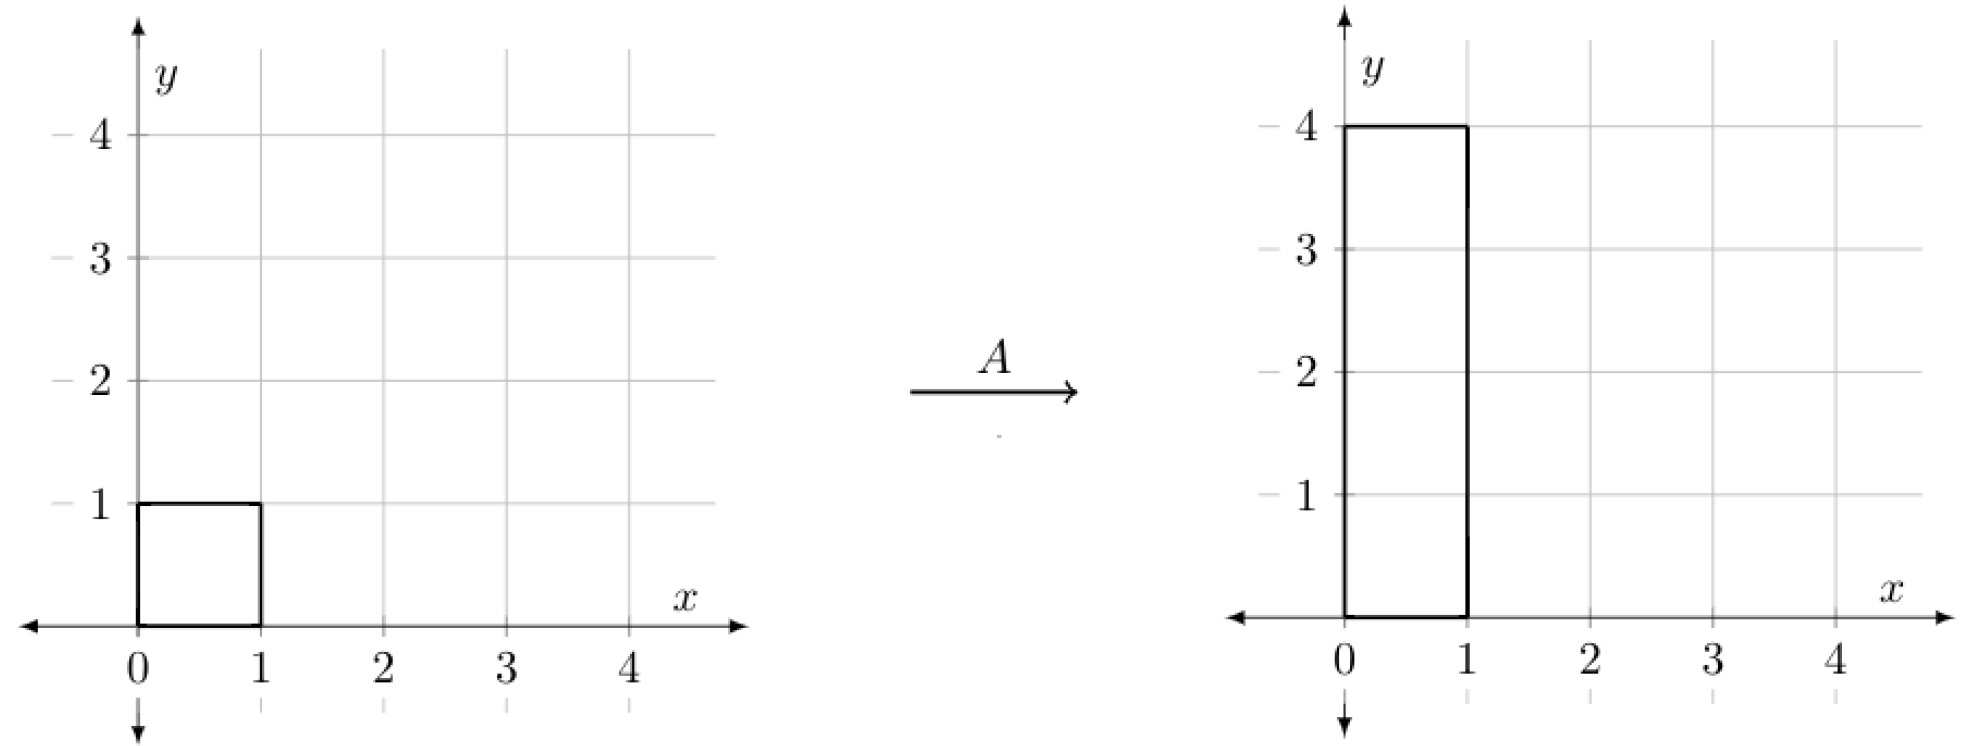
\includegraphics[scale=.5]{TransformationA.jpg}
\end{center}
Donc : la multiplication par une matrice diagonale est facile à comprendre.

	\item Qu'en est-il de la multiplication par $B = \scriptsize\mat{3&-1\\-2&2}$ ?  En l'appliquant
au m\^eme carré unitaire dont les sommets sont $(0,0)$, $(0,1)$, $(1,0)$, $(1,1)$, on obtient le parallélogramme dont les sommets sont :
$$
(0,0), (-1,2), (3,-2), (2,0)\,.
$$
\begin{center}
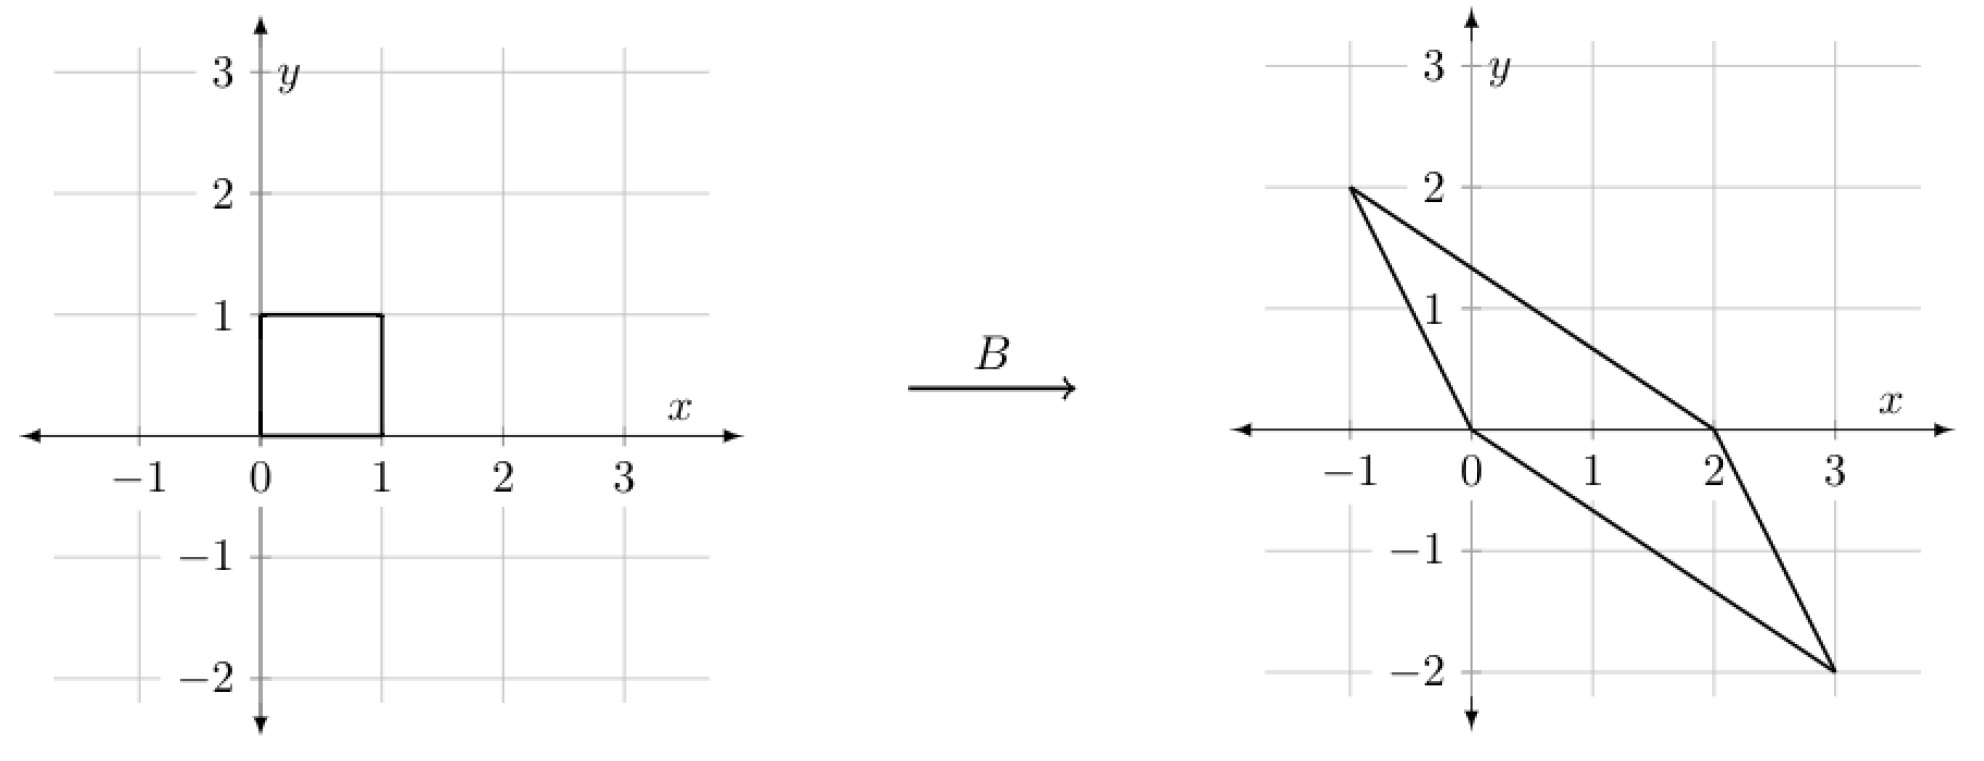
\includegraphics[scale=.5]{TransformationB1.jpg}
\end{center}
\end{enumerate}
Pourquoi y a-t-il une telle différence ?  
Le secret réside en fait dans les vecteurs propres. 
\begin{enumerate}[(1')]
	\item La matrice $A$ admet deux valeurs propres distinctes : $\lambda = 1$, à laquelle on peut associer le vecteur propre $(1,0)$, et $\lambda =4$, à laquelle on peut associer le vecteur propre $(0,1)$. Les espaces propres correspondent en fait aux axes canoniques : l'axe des $x$ et l'axe des $y$. C'est pour cela que la multiplication par $A$ transforme de manière aussi élégante le carré unitaire : parce que le carré unitaire a chacun de ses côtés parallèle à l'un des axes $x$ ou $y$, donc parallèle aux espaces propres.
	\item Faisons pareil pour $B$ : trouvons les axes avec lesquels il faut que les segments du dessin de départ soient parallèles pour mieux comprendre la transformation induite par $B$. La matrice $B$ admet deux valeurs propres distinctes : $\lambda = 1$, à laquelle on peut associer le vecteur propre $(1,2)$, et $\lambda =4$, à laquelle on peut associer le vecteur propre $(-1,1)$.
Considérons le parallélogramme dont les sommets sont ces deux vecteurs propres, l'origine, et le 4e sommet $(0,3)$:
$$
(0,0), (1,2), (-1,1), (0,3)\,.
$$
Alors, après multiplication par $B$, on obtient le parallélogramme :
$$
(0,0), (1,2), (-4,4), (-3, 6)\,.
$$
C'est le même parallélogramme, mais «~étiré~» 
d'un facteur de $4$ dans la direction $(-1,1)$. 
\begin{center}
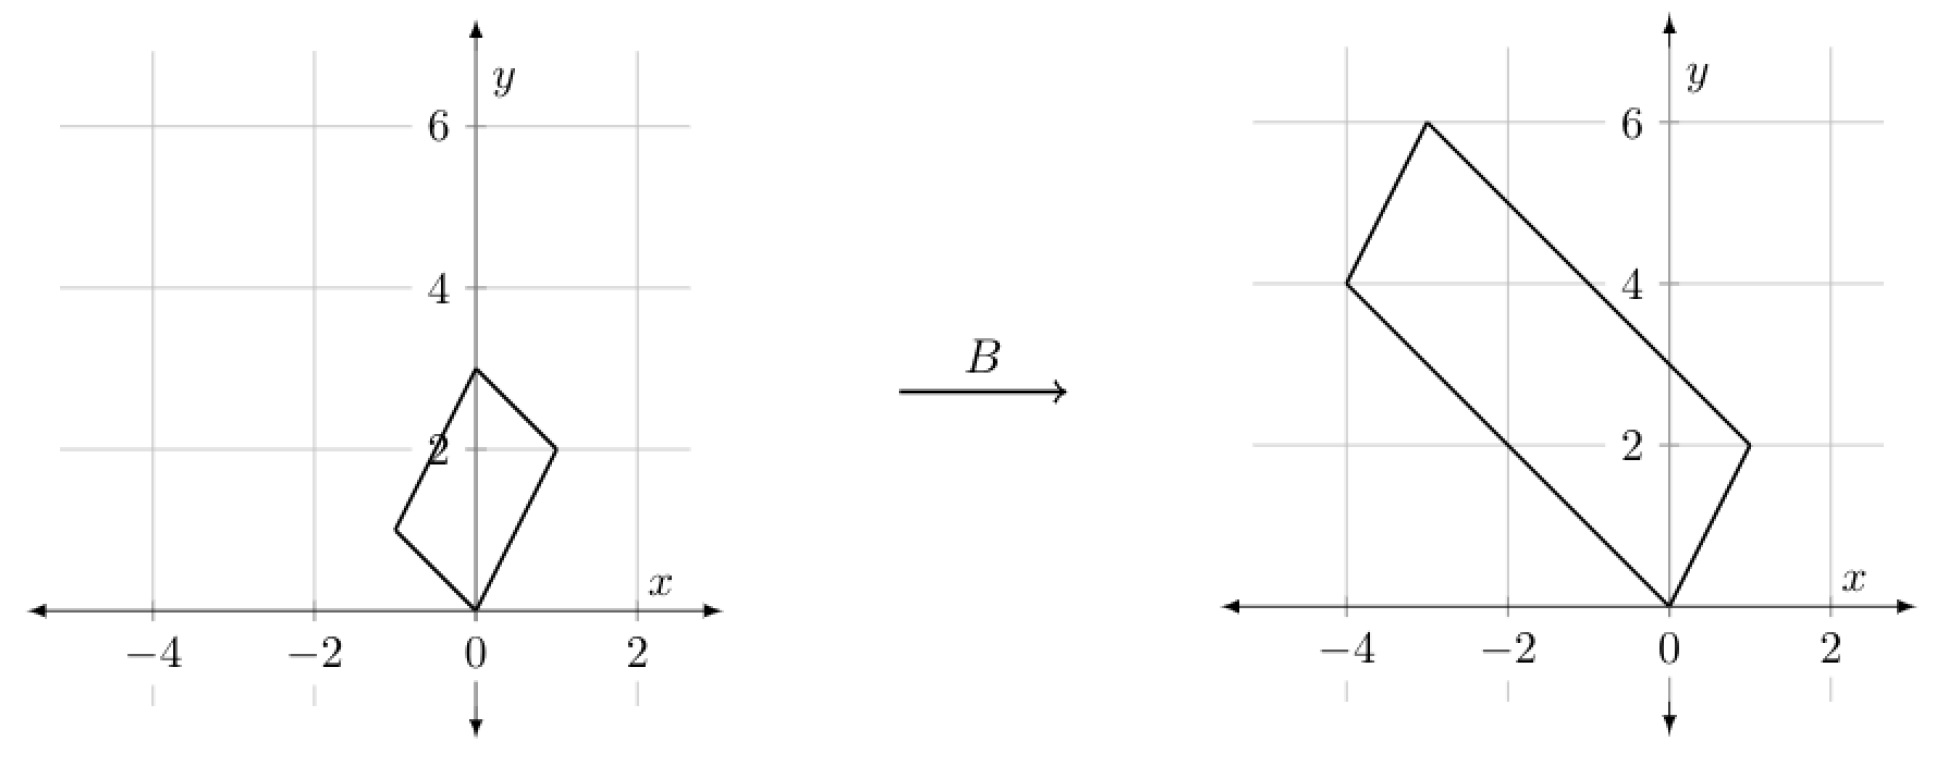
\includegraphics[scale=.5]{TransformationB2.jpg}
\end{center}
En fait, on voit alors que la matrice $B$ agit de la même manière que la matrice $A$, mais avec un angle différent ! Dans les deux cas, un axe est laissé intact, et l'autre est «~étiré~» d'un facteur $4$.
Par la même occasion, on comprend mieux aussi ce qui arrive à notre brave carr\'e unitaire dans le 2e schéma : il
a été étiré et déformé le long de deux droites différentes des axes $x$ et $y$, c'est pour cela qu'on obtenait un parallélogramme.
\end{enumerate}
Moralit\'e : les vecteurs propres sont le secret pour comprendre
la géométrie de la multiplication par une matrice.
\end{myexample}

Le fait de considérer une matrice $A$ de cette manière comme une transformation --- plus précisément comme une \stress{transformation linéaire} --- est un principe fondamental, avec de multiples applications notamment pour les systèmes dynamiques discrets et les processus de Markov\footnote{Recherchez sur le web  \og Chaînes de Markov\ \fg.} en probabilité.


Dans le prochain chapitre, ce que nous voulons faire, c'est explorer cette idée de transformations linéaires plus en détail
et revenir sur l'image qui illustre le lien entre le noyau $\ker(A)$ et l'espace image $\im(A)$ via une \emph{transformation} de
$\R^n$ dans $\R^m$ (la transformation étant : la multiplication par $A$, qui a $\xx\in\R^n$ associe $A\xx\in\R^m$).



